% % !TeX program = xelatex
% !TeX spellcheck = es_ES
% !TeX encoding = utf8

\documentclass[onecolumn,10pt,titlepage,a4paper]{article}

\usepackage[a4paper,top=2.5cm,bottom=2cm,left=2cm,right=2cm,marginparwidth=1.75cm,headheight=28pt]{geometry}
% Formateo para castellano
%\usepackage[utf8]{inputenc}
\usepackage[spanish,mexico]{babel}
%\usepackage{natbib}


\newcommand{\celsius}{^\circ \mathrm{C}}
\newcommand{\air}{{\mathrm{humo}}}
%Bibliografía

% Simbolos para notas de pie
\usepackage[symbol]{footmisc}
\renewcommand*{\thefootnote}{\fnsymbol{footnote}}

% \renewcommand{\thefootnote}{\fnsymbol{footnote}}
% \footnote[num]{text}

% \pagestyle{myheading}
% \markright{Mi Documento \hfill Mi nombre \hfi}
%
\usepackage{fancyhdr,framed}
\setlength{\headheight}{15.2pt}
\pagestyle{fancy}
\lhead{Elementos Finitos II - 31.92 \\ Patricio Whittingslow -- 55423}
\chead{TP 2}


%\usepackage{subcaption}

% Para el entorno align


% Multiples columnas para glosario
\usepackage{multicol}

%Figuras y subtitulos
\usepackage{graphicx}
\usepackage{caption,subcaption}
\usepackage{hyperref}
\hypersetup{
    colorlinks,
    citecolor=black,
    filecolor=black,
    linkcolor=black,
    urlcolor=black
}
\usepackage[utopia,expert]{mathdesign} %Opcion "expert" para no romperme las smallcaps de helvetica. 
\usepackage{amsmath}

\newcommand{\rmfont}[1]{{\fontfamily{ptm}\selectfont%
		#1}}
\newcommand{\rmfontbf}[1]{{\fontfamily{ptm}\selectfont%
		\textbf{#1}}}
\newcommand{\rmfontsc}[1]{{\fontfamily{ptm}\selectfont%
		\textsc{#1}}}
    
\newcommand{\Matlab}{\rmfont{\sc Matlab}}
    \newcommand{\Adina}{{\sc ADINA}}
    \newcommand{\refp}[1]{(\ref{#1})}
    \newcommand{\unspace}{\!\!\!\!\!\!\!\!\!\!\!\!\!\!\!\!\!\!\!\!}
    \newcommand{\ms}{\ \ \ } %Matrix Spacing
    \newcommand{\di}{\textrm{d}}
    \newcommand{\jac}{\rmfontbf{J}}
    \newcommand{\Djac}{|\;\jac\;|}
    \newcommand{\dNi}{\di N_i}
    \newcommand{\sigmab}{\boldsymbol{\sigma}}
    \newcommand{\varepsilonb}{\boldsymbol{\varepsilon}}
    \newcommand{\Phib}{\boldsymbol{\Phi}}
    \newcommand{\CPhi}{\boldsymbol{\{ } \Phi \boldsymbol{\} }}
    \newcommand{\Mme}[1]{\boldsymbol{[}\mathbf{#1} \boldsymbol{]}}
    \newcommand{\Rme}[1]{\boldsymbol{\lfloor}\mathbf{#1} \boldsymbol{\rfloor}}
    \newcommand{\Cme}[1]{\boldsymbol{\{ }\mathbf{#1} \boldsymbol{\}} }
    \newcommand{\MB}{\Mme{B}}
    \newcommand{\MN}{\Mme{N}}
    \newcommand{\ME}{\Mme{E}}
    \newcommand{\Mk}{\Mme{k}}
    \newcommand{\MA}{\Mme{A}}
    \newcommand{\radial}{r}
    \newcommand{\eff}{f}
%Helvetica
\renewcommand{\familydefault}{\sfdefault}
\usepackage[scaled=1]{helvet}
\usepackage[format=plain,
            labelfont={bf,it},
            textfont=it]{caption}
%\usepackage[T1]{fontenc}
%--------------------------------------


\usepackage{siunitx}
\newcommand{\glossentry}[2]{$#1\ $ \indent #2 \par \vspace{.4cm} }
\newcommand{\adm}{\textrm{adm}}
\renewcommand\thepart{\Alph{part}}

\title{Informe Técnico - ITBA}

\author{Patricio Whittingslow}
%========================> Comienza Documento
\begin{document}
\begin{titlepage}
	\centering
	
	{ \large Instituto Tecnológico de Buenos Aires  \par }
	\vspace{2cm}
	{\Large \scshape Elementos Finitos II - 31.92 \par}
	\vspace{2cm}
	{\Huge \scshape Estudio de vibraciones de una viga y un motor utilizando el método de elementos finitos\par }
	\vspace{.5cm}
	{\Large  \par}
	\vspace{2cm}
	{\large \bf Autor \par}
	\vspace{.5cm}
	\textsc{\large Patricio Whittingslow -- 55423}
	\vspace{2cm}
	{\par \large Fecha de realización: \today \par}
	\vspace{1cm}
	{\large Fecha de entrega: .......................................\par}
	\vspace{\fill}
	{\large Firma del docente: .......................................}
	\vspace{\fill}
	\begin{figure}[htb!]
		\centering
		
\includegraphics[width=6cm]{fig/logoitba.png}
	\end{figure}
\end{titlepage}




\begin{multicols}{2}
	\section*{Glosario}
	\glossentry{\Cme{R}}{Vector de cargas externas.}
	\glossentry{\Mme{K}}{Matriz de rigidez.}
	\glossentry{\Mme{M}}{Matriz de masa.}
	\glossentry{\Cme{D}}{Vector de desplazamientos.}
	\glossentry{\chi}{Razón entre la frecuencia de excitación y la frecuencia natural del modo estudiado.}
	\glossentry{\Mme{C}}{Matriz de amortiguamiento.}
\end{multicols}

\setcounter{section}{-1}

\tableofcontents

\section{Introducción Teórica}
Cuando se tiene una carga dependiente del tiempo la respuesta estructural también lo es. En el caso que sea un problema cuasiestático la resolución se puede hacer para los instantes de tiempos interesantes. Caso contrario se precisa efectuar un \textit{análisis dinámico}.
\[
\text{Cuasiestático:}\quad \Mme{K}\Cme{D} = \Cme{R} \longrightarrow \text{Dinámico:} \quad 
\Mme{M} \Cme{\ddot{D}} + \Mme{C}\Cme{\dot{D}} + \Mme{K}\Cme{D} = \Cme{R}	
\]
donde el termino $\Mme{K}\Cme{D}$ suele ser referido como las \textit{fuerzas internas}, y $\Cme{R}$ siendo las \textit{fuerzas externas}.

El análisis dinámico busca la forma de deformación del sistema cuando este se encuentra excitado por cargas a una frecuencia cercana a la natural. La respuesta en deformación del sistema con una carga cíclica puede ser menor o mayor que con cargas estáticas de misma magnitud máxima, pero cuando la frecuencia de carga se acerca a la natural las deformaciones serán mucho mayor. 

Debido a este último punto es de sumo interés conocer la frecuencia natural de un sistema que tiene la posibilidad de someterse a una carga cíclica. Incluso puede ser de gran utilidad conocer el modo de deformación para entender como el sistema almacena energía.


\part{Estudio de Motor}
\setcounter{section}{0}
\section{Problema}

\begin{itemize}
	\item Se precisa proponer un modelo para la estructura y representar gráficamente.
	\item Efectuar análisis modal y dimensionar las vigas del basamento. Considerar desplazamiento de $10$mm y $\omega_{\mathrm{exc}}=600\mathrm{rpm}$.
	\item Proponer un diseño alternativo superador teórico dejando de lado la perspectiva económica. Este diseño debe reducir cargas transmitidas y los desplazamientos del equipo.
\end{itemize}



\begin{figure}[htb!]
	\centering
	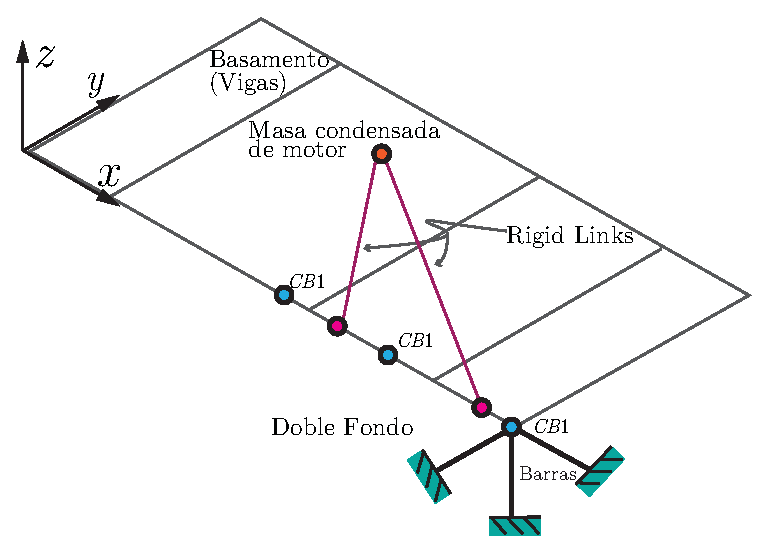
\includegraphics[width=0.6\textwidth]{fig/modelomotor.eps}
	\caption{Modelo del motor a grandes rasgos. El problema fue resuelto en \Matlab.}
	\label{fig:modelomotor}
\end{figure}

\section{Método}
El problema se resuelve en \Matlab{} utilizando el método de elementos finitos.

Elementos usados
\begin{itemize}
	\item Elemento masa 0D para masa puntual (sin rigidez)
	\item Elementos viga Timoshenko con masa consistente para basamento
	\item Elementos Barra simples para Rigid links con rigidez $\num{1e8}$ \si{\newton \per \meter} con matriz de masa nula
	\item Elemento resorte para los bulones (nodos azules con $CB1$ en la figura \ref{fig:modelomotor}) con rigidez longitudinal de bulón $k_b$ en dirección $z$ y rigidez $\frac{k_b}{10}$ en $x$ e $y$ para representar el efecto de separar el motor del doble fondo con una resina.
\end{itemize}

Para el mallado se desarrollo un programa que cree los nodos y una los elementos automáticamente, tomando como input del usuario el tamaño nominal de los elementos viga. En la figura \ref{fig:modelobasamento} se ve el resultado de dicho programa con tamaño de elemento \textit{máximo.} Para la constante torsional $J_\tau$ se utilizó una formula aproximada para secciones rectangulares \eqref{eq:torsionalConstant}\footnote{Obtenido del libro \cite{young2002roark}}

\begin{equation} \label{eq:torsionalConstant}
J_{\tau}=h \cdot b^{3} \cdot\left(\frac{1}{3}-0,21 \cdot \frac{b}{h} \cdot\left(1-\frac{b^{4}}{12 \cdot h^{4}}\right)\right)
\end{equation}
donde $b$ es el lado corto y $h$ el lado largo.


\begin{figure}[htb!]
	\centering
	\begin{subfigure}{0.49\textwidth}
		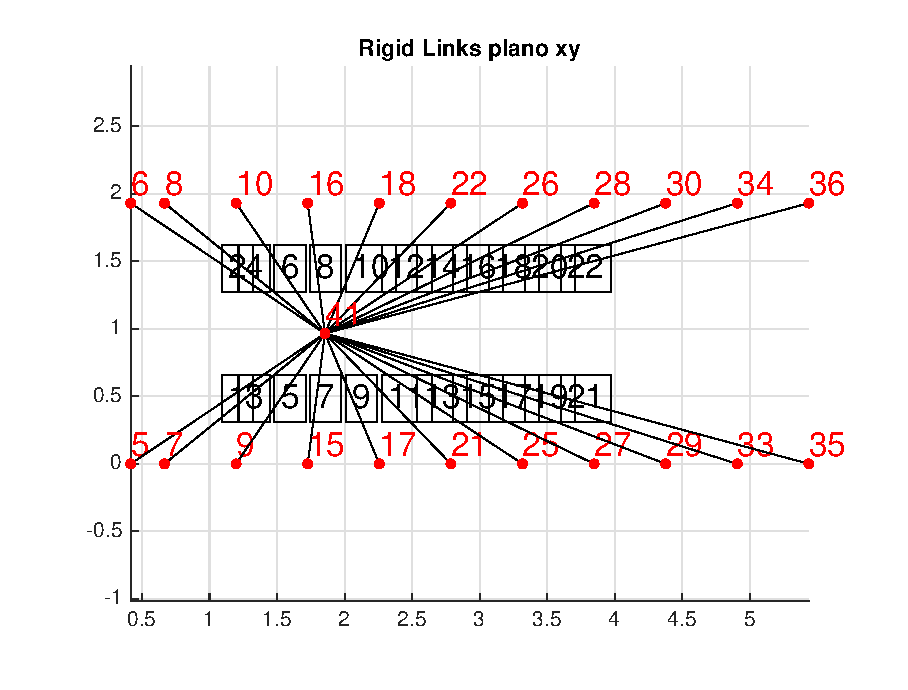
\includegraphics[width=\linewidth]{fig/modelRLxy.eps}
		\caption{Rigid links. Vista en plano $x\!y$.}
		\label{fig:modeloRLxy}
	\end{subfigure}
	\begin{subfigure}{0.49\textwidth}
		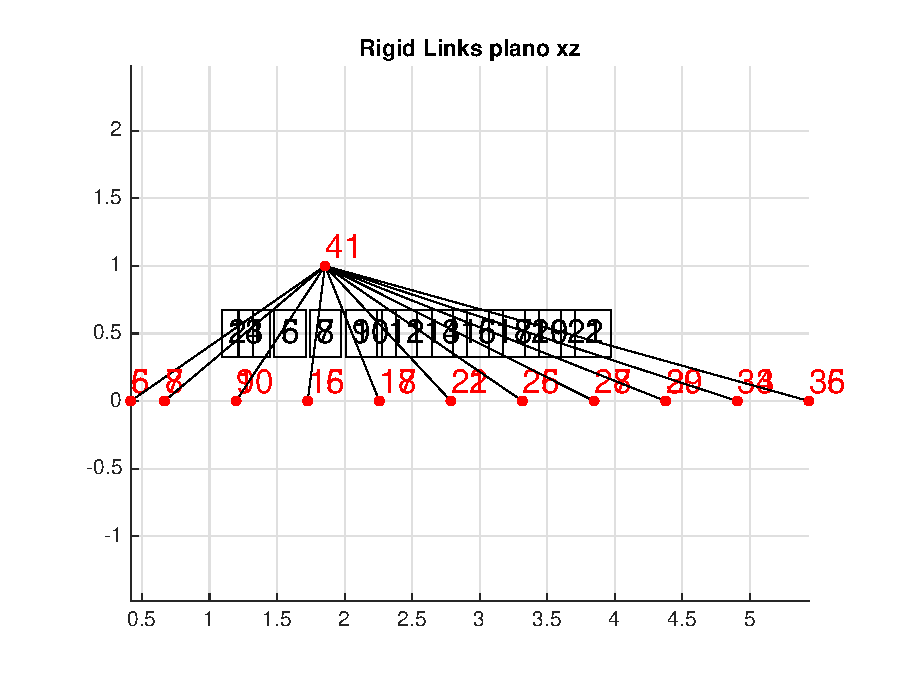
\includegraphics[width=\linewidth]{fig/modelRLxz.eps}
		\caption{Rigid links. Vista en plano $x\!z$.}
		\label{fig:modeloRLxz}
	\end{subfigure}
\end{figure}

\begin{figure}[htb!]
	\centering
	\includegraphics[width=0.8\textwidth]{fig/modelbasamento.eps}
	\caption{Modelo Basamento. Vista en plano $x\!y$.Tome en cuenta que los nodos numerados no necesariamente tienen que coincidir con figura de rigid links.}
	\label{fig:modelobasamento}
\end{figure}

\subsection*{Selección de parámetros}
Para un primer análisis se fijaron las distancias entre los bulones de tal forma como para que tengan el mismo espacio entre ellos. Se resuelve el problema para solicitaciones cuasiestáticas (peso de motor) para obtener la optima posición de los soportes en $y$.


\begin{table}[htb!]
	\centering
	\begin{tabular}{lllll}
		& 1 & 2 & 3 & 4 \\ \hline
		Uniones Abulonadas& 0,097 \si{\meter}  & 1,897 \si{ \meter} & 3,697 \si{ \meter} & 5,567 \si{ \meter} \\
		Soportes en $y$& 0,797 \si{\meter}  &1,787\si{\meter}   & 2,587 \si{\meter}  &  \\
	\end{tabular}
\caption{Posición en $x$ de los nodos correspondientes a los bulones que unen doble fondo con basamento y las vigas estructurales en $y$.}
\end{table}

Para dimensionar las vigas del basamento se comenzó resolviendo el sistema cuasiestático donde la única carga es el peso del motor. Esto dará un rango de dimensiones inicial para trabajar el problema dinamicamente. Luego del dimensionado cuasiestático (todas las vigas tienen las mismas dimensiones para simplificar el problema) iteramos variando $h$ y $b$ para todas las vigas. El amortiguamiento del sistema está controlado por la resina en los bulones. Se decidió modelar esto como un amortiguamiento global de $\dampfact = 0,1$ en un análisis con amortiguamiento modal. La excitación $\omega_{\mathrm{exc}}$ es de 600 rpm y se calcula la amplitud de excitación según un desplazamiento de $10$mm sobre la masa puntual en la dirección $z$.

Por último se va efectuar un análisis con amortiguamiento proporcional usando la primer frecuencia natural del sistema como $\omega_1$ y $\omega_2 = 1,15 \omega_{\mathrm{exc}}$. Se amortiguan estos modos con $\dampfact_{1}=0,06$ y $\dampfact_2=0,2$, respectivamente. El desarrollo de esta formulación queda detallada en la parte B de este informe. 

\section{Resultados del dimensionamiento}

Se ve una diferencia importante en la suavidad entre las superficies que representan la amplitud en función de $h$ y $b$ según el tipo de amortiguamiento usado. Sin embargo, ambas tienen una interpretación concreta.

El amortiguamiento modal impone un amortiguamiento global. Esto implica que todo el espectro de frecuencias naturales entra en juego para una excitación dada. Al cambiar la rigidez del sistema su estructura tendrá mayor resistencia ante el movimiento del motor.

Por otro lado el amortiguamiento proporcional discrimina según la frecuencia. Lo que puede estar sucediendo al momento de cambiar las dimensiones de la viga es que cambiamos cual frecuencia natural domina. En las zonas de amplitud máxima puede ser que dominen las frecuencias cercanas a $\omega_{\mathrm{exc}}$ mientras que en los valles la rigidez de las vigas en conjunto es lo suficientemente diferente para que cambie el modo de deformación.



Se elige entonces una viga rectangular $h=6,5\si{\milli \meter}$ y $b=8\si{\milli \meter}$


\begin{figure}[htb!]
	\centering
	\begin{subfigure}{0.47\textwidth}
		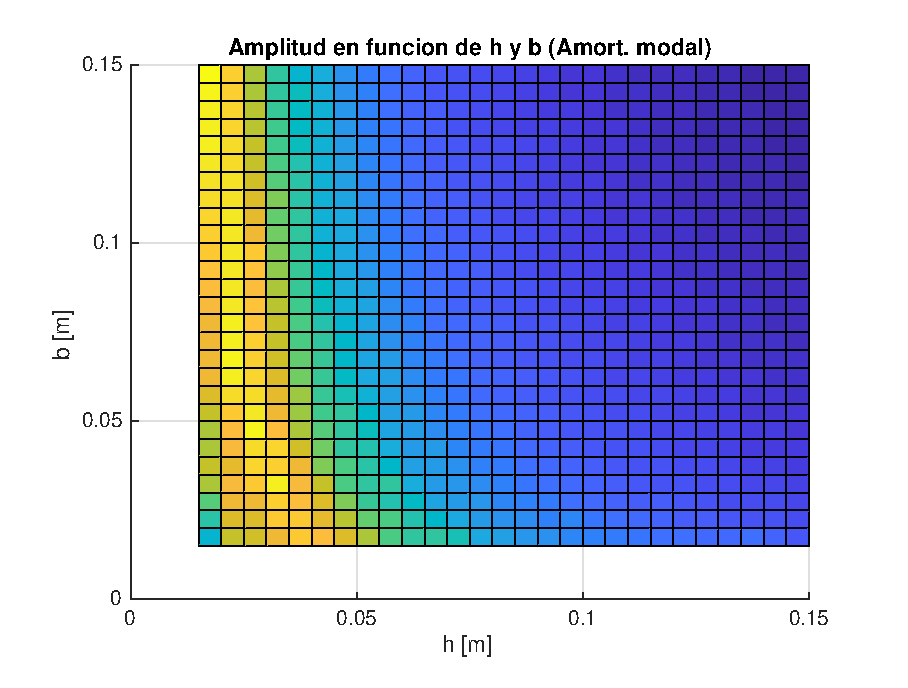
\includegraphics[width=\linewidth]{fig/amplitudVshb.eps}
		\caption{Amplitud en función de las dimensiones $h$ y $b$ de la viga considerando desplazamiento $d=10$mm. Amarillo es mayor, azul es menor.}
		\label{fig:amplitudVshb}
	\end{subfigure}
\hfill
	\begin{subfigure}{0.5\textwidth}
		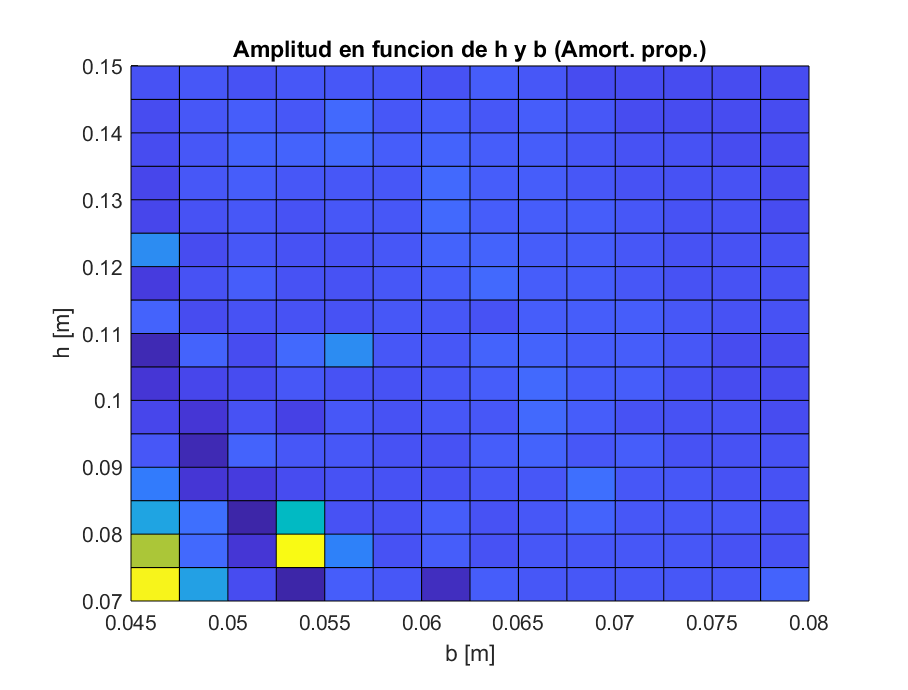
\includegraphics[width=\linewidth]{fig/amplitudVshbProp.eps}
		\caption{Amplitud en función de las dimensiones $h$ y $b$ de la viga en un análisis modal considerando una fuerza constante. Amarillo es mayor, azul es menor. Longitud de elemento caracteristica $L_e=0,1$m.}
		\label{fig:amplitudVshbProp}
	\end{subfigure}
\end{figure}

\begin{figure}
	\centering
			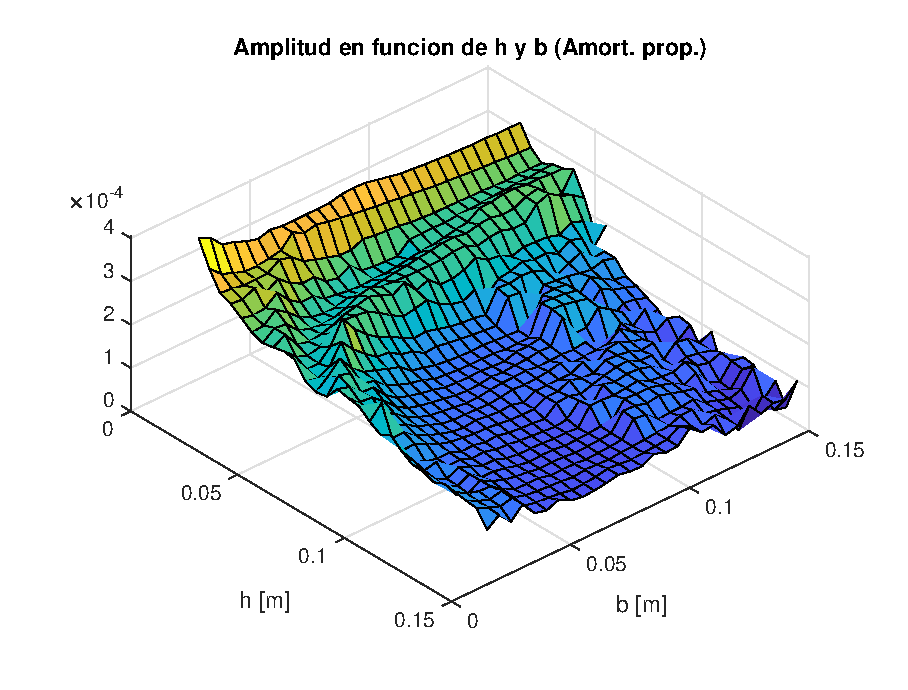
\includegraphics[width=0.7\linewidth]{fig/amplitudVshbPropRefinado.eps}
	\caption{Similar a figura \ref{fig:amplitudVshbProp} pero con refinamiento de elementos global. Longitud de elemento caracteristica $L_e=0,05$m.}
	\label{fig:amplitudVshbPropref}
\end{figure}

\section{Optimización teórica}


\clearpage
\part{Viga Empotrada}

\setcounter{section}{0}
\section{Problema}
Hallar para el problema descrito en la figura \ref{fig:enunciado}:
\begin{itemize}
	\item Frecuencias Naturales
	\item Amortiguamiento modal y proporcional
	\item Carga armónica
	\item \textit{Frecuencia de Barrido}
\end{itemize}

\begin{figure}[htb!]
	\centering
	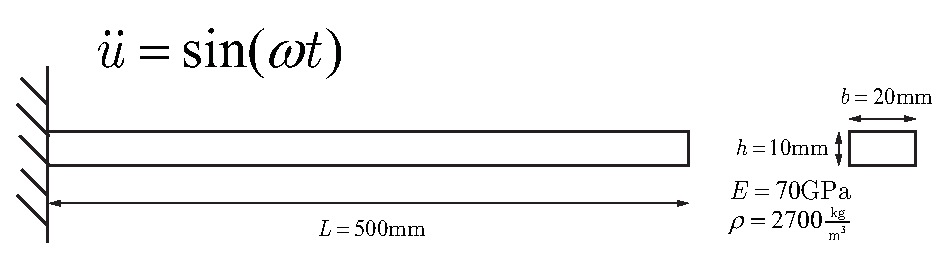
\includegraphics[width=0.6\textwidth]{fig/enunciado.eps}
	\caption{Se resolvió para una viga de aluminio empotrada excitada por una aceleración uniforme.}\label{fig:enunciado}
\end{figure}
Cabe destacar que el enunciado original otorgado por la cátedra sugería usar para la aceleración excitadora $\ddot{u}=\sin (\Omega x)$, el cual nos daría un sistema cuasiestático poco interesante.\footnote{a no ser que $\Omega$ esté en función del tiempo y no se haya especificado}

\section{Método}
Se resuelve el problema por método de los elementos finitos utilizando vigas de dos nodos. Cada nodo tiene dos grados de libertad, $v$ como el desplazamiento en $y$ y $\theta$ siendo el giro de la viga en el plano $x\!y$.

La matriz de masa usada es \textit{consistente}. Esta y la matriz de rigidez toman la forma: \cite[p.379]{cook2007concepts}
\[
\Mme{m}_{\mathrm{viga}}=\frac{\rho A L}{420}\left[\begin{array}{cccc} 156 & 22\,\mathrm{L} & 54 & -13\,\mathrm{L}\\ 22\,\mathrm{L} & 4\,{\mathrm{L}}^2 & 13\,\mathrm{L} & -3\,{\mathrm{L}}^2\\ 54 & 13\,\mathrm{L} & 156 & -22\,\mathrm{L}\\ -13\,\mathrm{L} & -3\,{\mathrm{L}}^2 & -22\,\mathrm{L} & 4\,{\mathrm{L}}^2 \end{array}\right] \qquad \qquad \Mme{k}_{\mathrm{viga}}=\frac{E I_z}{L^3} \left[\begin{array}{cccc} 12 & 6\,L & -12 & 6\,L\\ 6\,L & 4\,L^2 & -6\,L & 2\,L^2\\ -12 & -6\,L & 12 & -6\,L\\ 6\,L & 2\,L^2 & -6\,L & 4\,L^2 \end{array}\right]
\]

Se resuelve el problema de autovalores para el sistema sin amortiguamiento \eqref{eq:eigenvalueproblem} y se obtienen las frecuencias naturales del sistema 

\begin{equation} \label{eq:eigenvalueproblem}
	\left( \Mme{K} - \omega^2 \Mme{M}\right)\Cme{D}= 0
\end{equation}

Luego se busca la respuesta armónica del sistema ante la carga conocida. Se propone estudiarlo con las autoformas.
\begin{equation} \label{eq:Zmodal}
	 \Cme{\boldsymbol{\ddot{\mathrm{Z}}}}+2\COmega \Cme{C\modal} \Cme{\boldsymbol{\dot{\mathrm{Z}}}} + \COmega^2 \Cme{Z} = \Cme{R\modal}
\end{equation}
cuya resolución resulta en 
\begin{equation}
	\Cme{Z} = \frac{\Cme{R\modal }}{{\COmega}^2 \sqrt{(1-\chi^2)^2 + (2 \Cme{C\modal} \chi)^2}}
\end{equation}
donde $\chi = \frac{\omega_{\mathrm{exc}}}{\Cme{\Omega}}$.

La formulación de \textbf{amortiguamiento modal} es la siguiente

\begin{equation}
\Mme{C\modal}=\left[ \begin{array}{ccc}{2 \omega_{n} \dampfact_{n}} & {0} & {0} \\ {0} & {\ddots} & {0} \\ {0} & {0} & {2 \omega_{1} \dampfact_{1}}\end{array}\right]
\end{equation}
eligiendosé un $\dampfact$ para cada modo.

La formulación de \textbf{amortiguamiento proporcional} propone una combinación lineal de la masa y la rigidez según
\begin{equation} \label{eq:proporcional}
\Mme{C\modal} = \Mme{\Phib}^T ( \alpha \Mme{M}+\beta \Mme{K})\Mme{\Phib} = \alpha \Mme{I} +\beta \Mme{\Omegab^2}
\end{equation}

Si se quiere estudiar un rango de frecuencias excitadoras tal que $\omega_{\mathrm{exc}}\in [\omega_1, \omega_2]$ y eligiendo dos valores de amortiguamiento para ambas frecuencias $\dampfact_1$ y $\dampfact_2$ se tiene: \cite{cook2007concepts}
\begin{align} \label{eq:alfabeta}
\alpha &= 2\omega_1 \omega_2 (\dampfact_1 \omega_2 -\dampfact_2 \omega_1)/(\omega_2^2 - \omega_1^2) \\ \beta &= 2(\dampfact_2\omega_2 -\dampfact_1 \omega_1)/(\omega_2^2 - \omega_1^2)
\end{align}

Se opta por estudiar el rango de amortiguamiento  $\varsigma\in \{0,05;\, 0,3\}$. Este es el rango inferior por donde se puede encontrar el amortiguamiento para problemas similares al enunciado.
\begin{itemize}
	\item Para el barrido de frecuencias de amortiguamiento proporcional se investigará el caso donde se elija $\varsigma_1=0,05$ fijo y variando $\varsigma_2$ para obtener las curvas de respuesta a frecuencia.
	\item El otro caso investigado será $\varsigma_2=0,3$ fijo variando así $\varsigma_1$.
\end{itemize}

\section{Resultados}
Las primeras tres frecuencias naturales obtenidas con una solución de 8 elementos.
\[
\Cme{\Omega} = \begin{Bmatrix}
\vdots \\
3627,5 \si{\, \radian \per \second}\\
1295,5 \si{\, \radian \per \second}\\
 206,7 \si{\, \radian \per \second}
\end{Bmatrix}=\begin{Bmatrix}
\vdots \\
577,3\, \textrm{hz}\\
206,2\, \textrm{hz}\\
32,9\, \textrm{hz} 
\end{Bmatrix}
\]

\begin{figure}[htb!] 
	\centering
	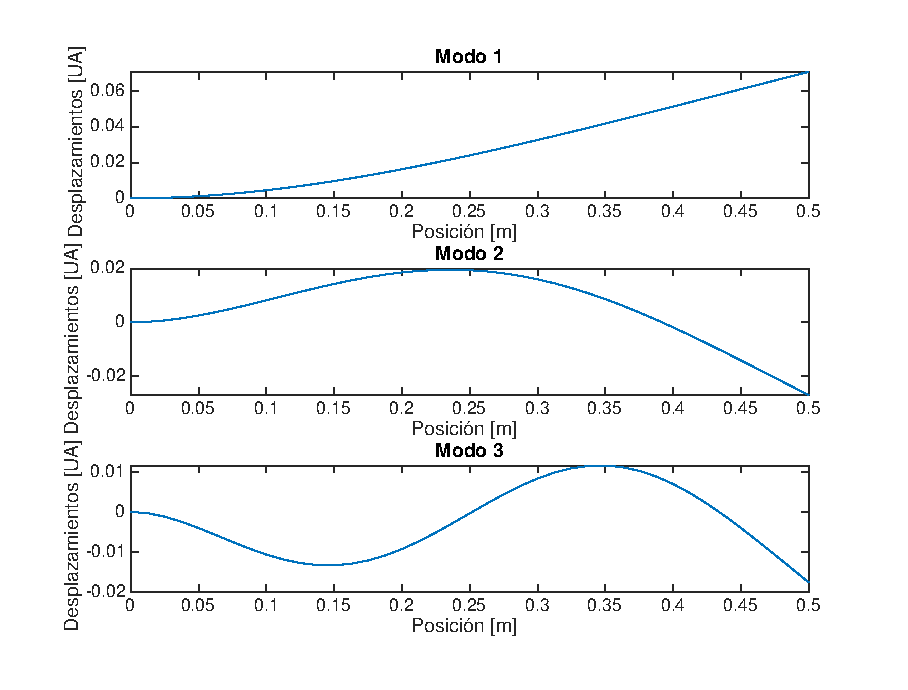
\includegraphics[width=1\textwidth]{fig/modos.eps}
	\caption{Modos de deformación para las frecuencias naturales. El modo 1 corresponde a la frecuencia más baja.}
	\label{fig:modos}
\end{figure}

\begin{figure}[htb!]
	\centering
	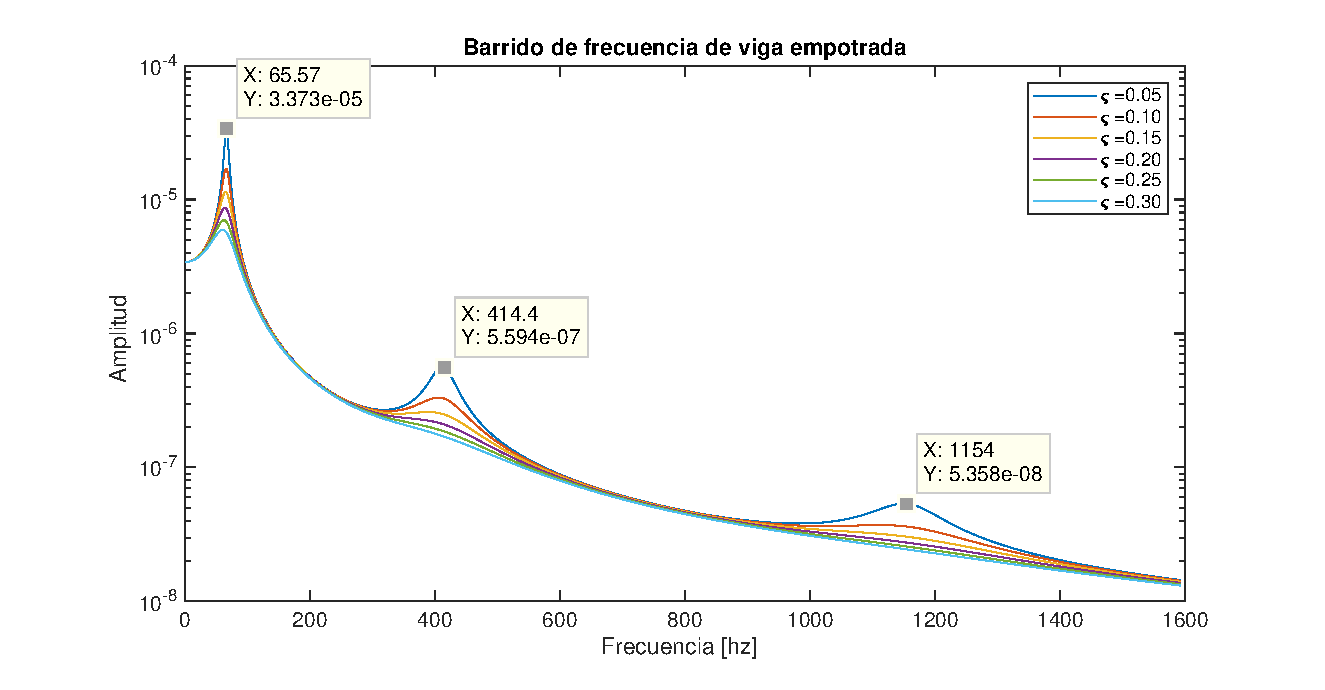
\includegraphics[width=1\textwidth]{fig/sinesweep.eps}
	\caption{Barrido de frecuencia \textbf{modal}. Valores de amplitud máxima recuadrados.}
	\label{fig:sinesweepmodal}
\end{figure}

\begin{figure}[htb!]
	\centering
	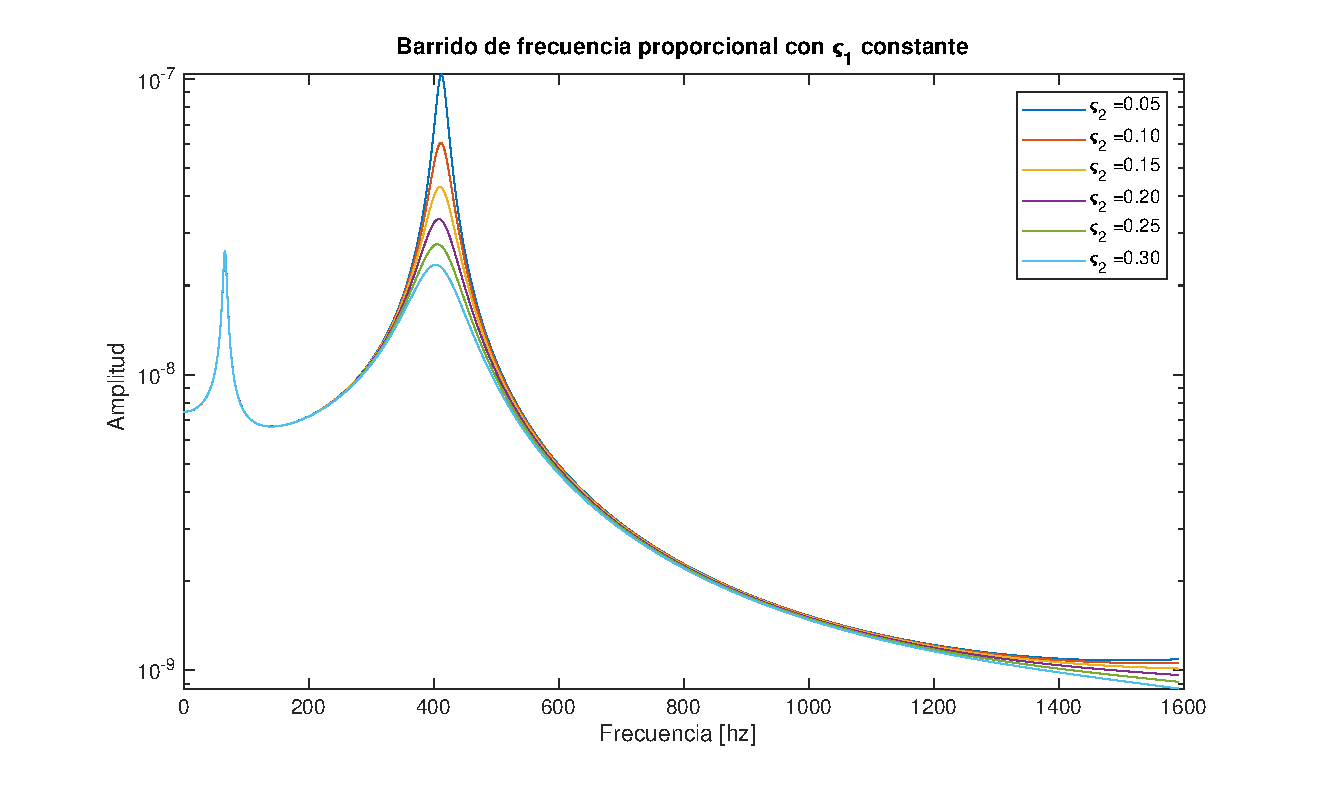
\includegraphics[width=1\textwidth]{fig/sinesweepprop1const.eps}
	\caption{Barrido de frecuencia \textbf{proporcional}.}
	\label{fig:sinesweepprop1}
\end{figure}

\begin{figure}[htb!]
	\centering
	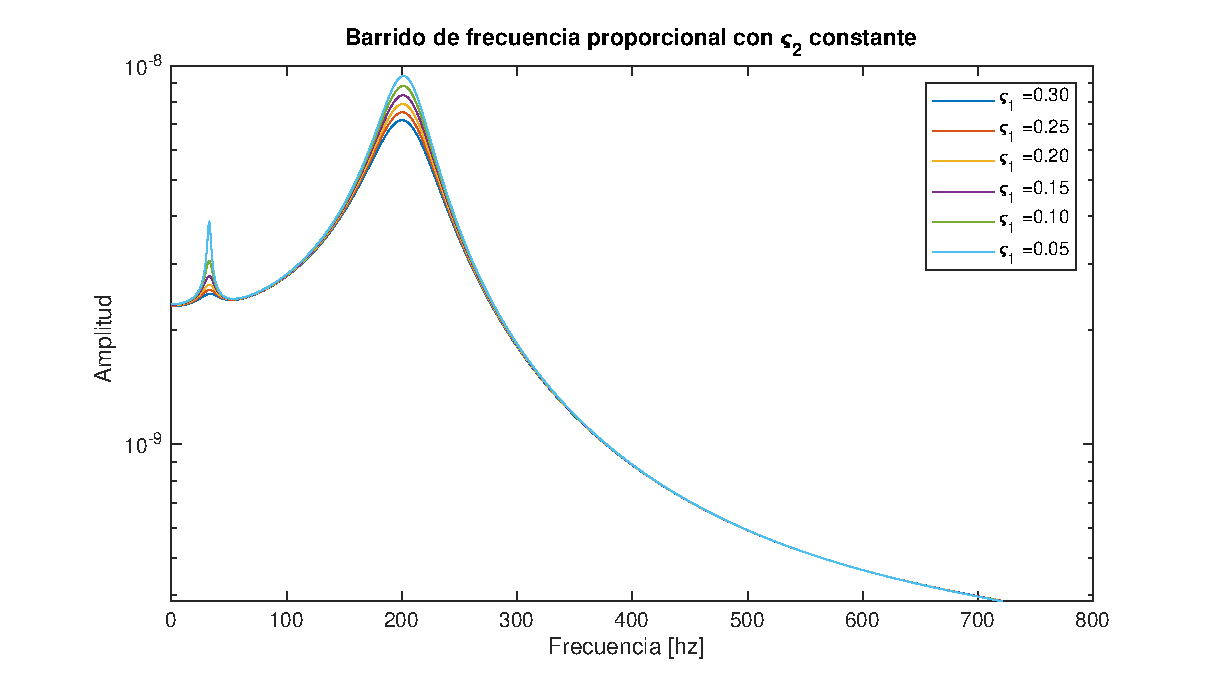
\includegraphics[width=1\textwidth]{fig/sinesweepprop2const.eps}
	\caption{Barrido de frecuencia \textbf{proporcional}.}
	\label{fig:sinesweepprop2}
\end{figure}





\clearpage
\section{Conclusiones}
Se informa al lector el hallazgo de la frecuencias naturales. Dichas frecuencias están separadas por un $\Delta \omega $ considerable. Esto es deseable para cuando se tenga una carga cíclica esta trabaje lejos de cualquier frecuencia natural, y si es posible, por debajo de todas. Dado que no se especifico ninguna característica técnica del problema, el gráfico \ref{fig:modos} es más una curiosidad. Las formas de los modos no están a escala ni tienen unidades, es solo la forma de respuesta. 

A medida que la frecuencia de excitación aumenta la \textit{amplitud del sistema disminuye}\footnote{Excepto en cercanías de una frecuencia natural} (ver figura \ref{fig:sinesweepmodal}). Es interesante pensar que si aumentara no tendría sentido buscar las frecuencias naturales porque estas son caracterizadas por un máximo de amplitud. Las curvas del barrido de frecuencia son decrecientes en lejanía de una frecuencia natural porque para una fuerza cíclica $F(t)=F_0\sin \omega t$ el tiempo que actúa en una dirección es inversamente proporcional a la frecuencia. Por ende la estructura no tiene tiempo para moverse lejos antes de que se invierta la dirección de la fuerza.

El efecto del amortiguamiento es reducir la amplitud cerca de la frecuencia natural. En la figura \ref{fig:sinesweepmodal} se puede apreciar el efecto claramente. Las siguientes dos figuras (\ref{fig:sinesweepprop1} y \ref{fig:sinesweepprop2}) tienen un nivel agregado de profundidad. Se estudia el efecto la \textit{fracción de amortiguamiento crítico} \cite{cook2007concepts} cuando se varía el amortiguamientos de los puntos borde del espectro de diseño. Como es de esperar para un valor mayor $\dampfact_1$ se amortiguarán a frecuencias más bajas sin afectar las de alta. De forma complementaria, si se aumenta $\dampfact_2$ la amplitud de la primera frecuencia natural no se ve afectada mientras que a frecuencias más altas se reduce la amplitud considerablemente.

 {\color{white} Humo: Lamento que si lo que buscabas con ese Ctrl+F era humo, no vasa a encontrar nada, solo esta nota pidiendo disculpas por la primera entrega. Perdón.}

\bibliography{labibliografia} % Indica archivo
\bibliographystyle{plainnat} 

\end{document}